\chapter{Giao diện}

\section{Console}
\code{app.exe} là chương trình menu (mục 0--12) trong cửa sổ dòng lệnh, có màu ANSI: xanh $=$ Sẵn sàng, vàng $=$ Đang mượn, đỏ $=$ Bảo trì hoặc quá hạn. Lớp \code{UI} chỉ gọi API công khai của \code{LabManager}, không chứa nghiệp vụ. Nhập sai (chữ thay số, ngoài khoảng, dòng trống) không làm treo chương trình: hỏi lại tối đa 3 lần rồi huỷ thao tác. Bảng căn cột theo số ký tự UTF-8 (không theo byte) để chữ có dấu không bị lệch cột.

\begin{figure}[H]
\centering
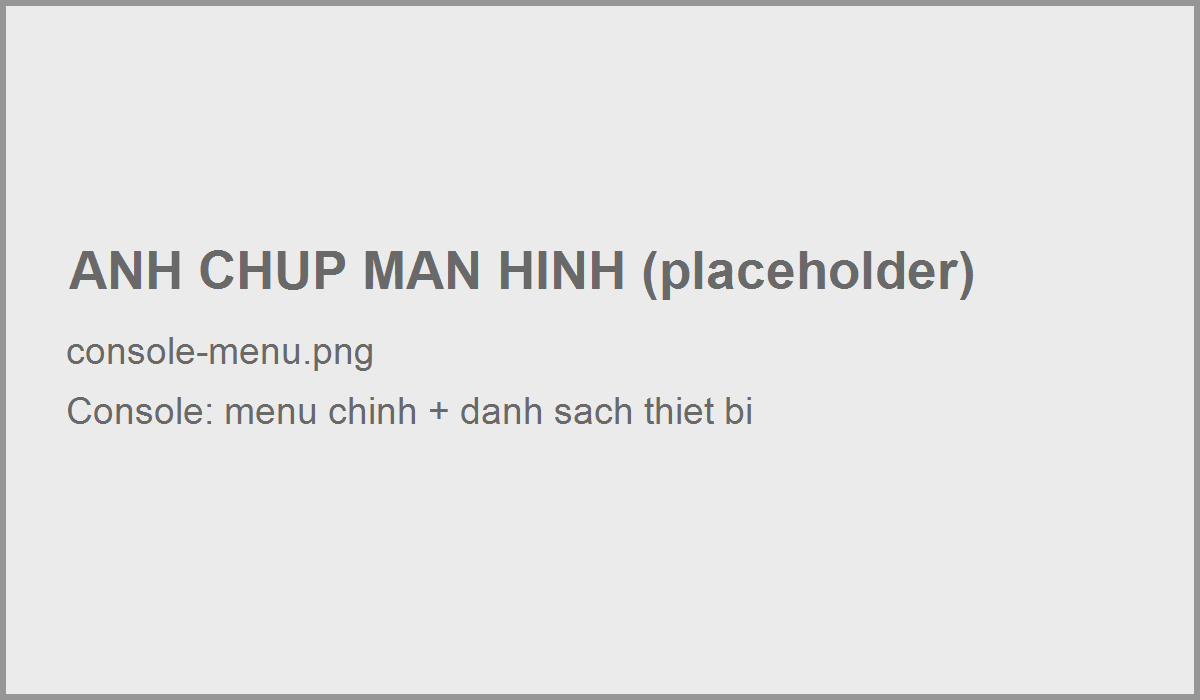
\includegraphics[width=0.92\textwidth]{figures/console-menu.png}
\caption{Console: menu chính và danh sách thiết bị}
\label{fig:console-menu}
\end{figure}

\begin{figure}[H]
\centering
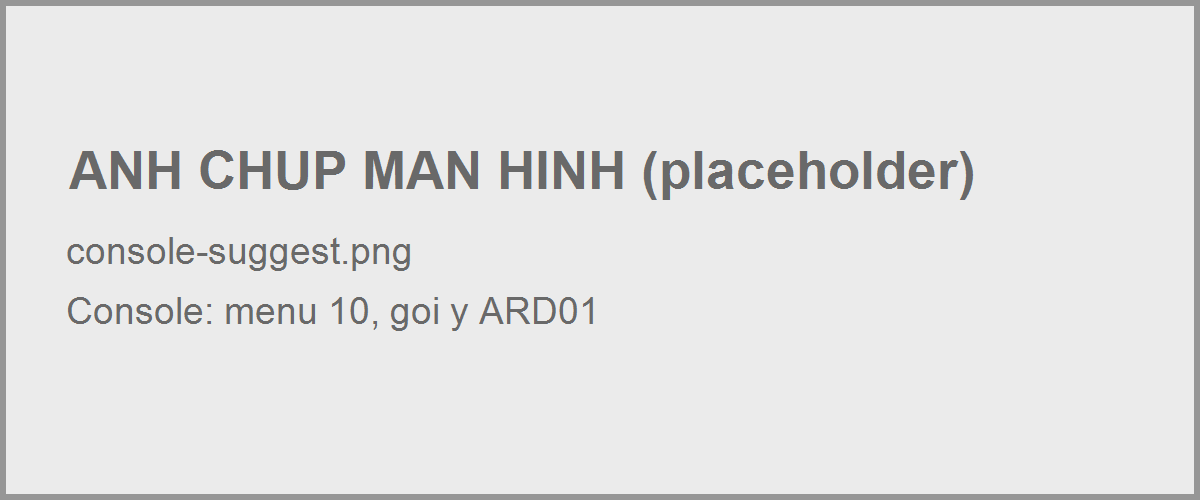
\includegraphics[width=0.92\textwidth]{figures/console-suggest.png}
\caption{Console: gợi ý thiết bị mượn kèm (menu 10)}
\label{fig:console-suggest}
\end{figure}

\section{Web}
\code{LabApp.exe} chạy máy chủ ở \code{127.0.0.1:8080}, phục vụ giao diện trong \code{web/} và API theo \code{docs/api.md}, rồi tự mở trình duyệt. Giao diện có bảy màn hình và một thanh đồng hồ giả lập có nút tua thời gian; mọi con số (quá hạn, gợi ý, vị trí hàng đợi) lấy từ API, không tính ở trình duyệt.

\subsection{Tổng quan}
Hiển thị tổng thiết bị, số đơn vị theo trạng thái, phiếu đang mở, phiếu quá hạn và phạt tạm tính, số người chờ/đang giữ, thiết bị mượn nhiều nhất.
\begin{figure}[H]
\centering
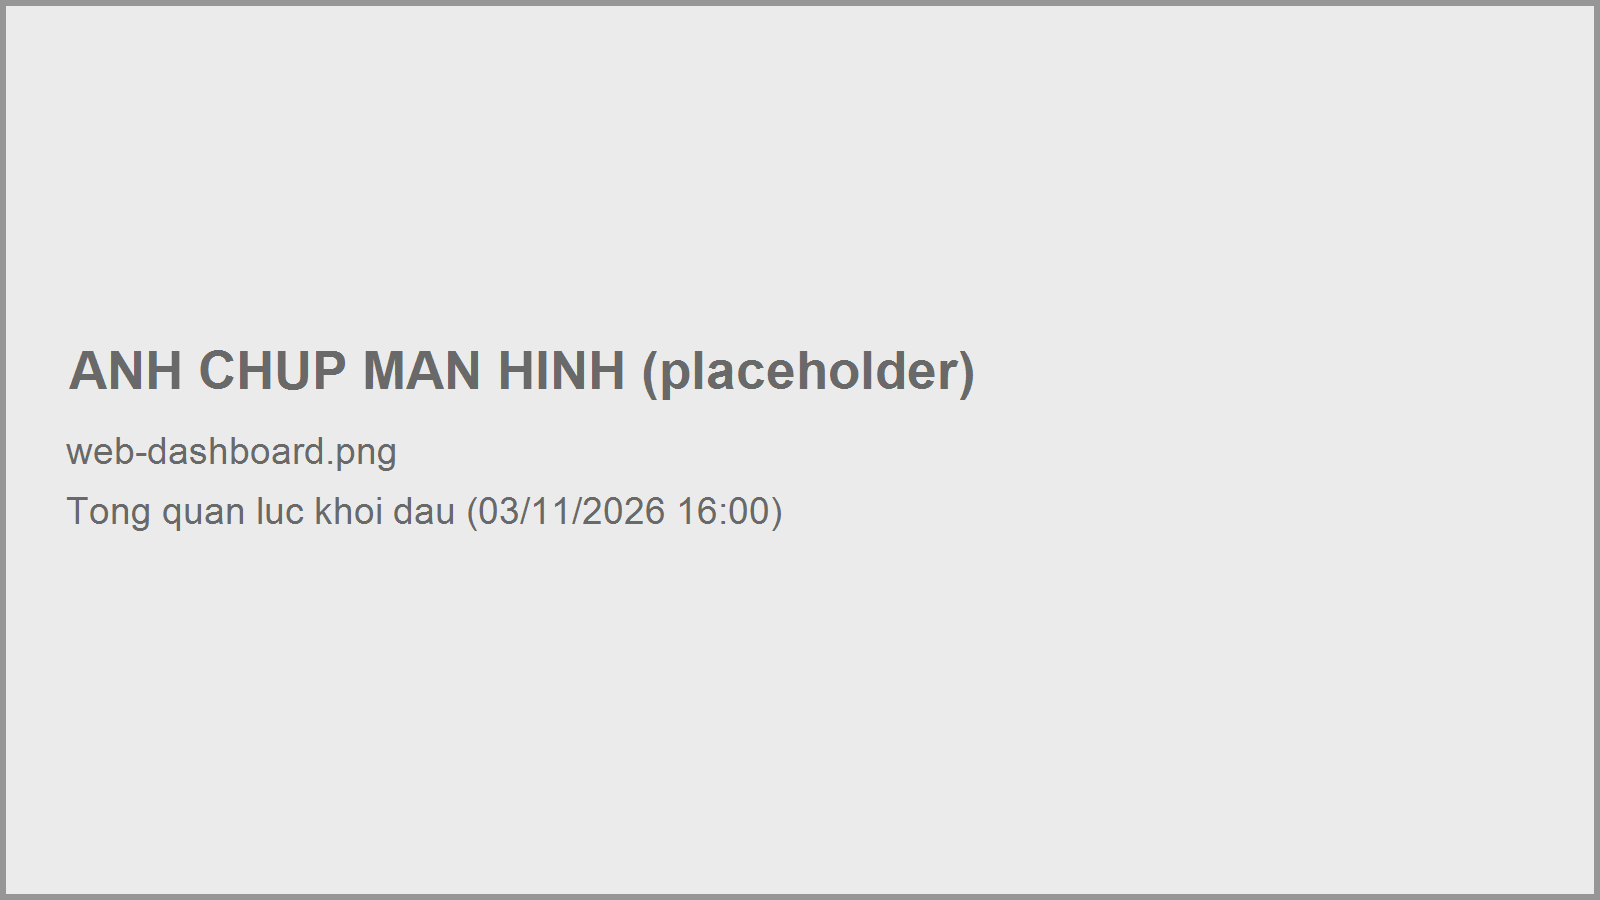
\includegraphics[width=0.95\textwidth]{figures/web-dashboard.png}
\caption{Màn Tổng quan ở trạng thái khởi đầu (03/11/2026 16:00)}
\label{fig:dashboard}
\end{figure}

\subsection{Thiết bị}
Danh sách thiết bị với thanh tỷ lệ \code{available/borrowed/onHold/maintenance} và trạng thái suy ra (M1); thêm, sửa, bảo trì, xoá.
\begin{figure}[H]
\centering
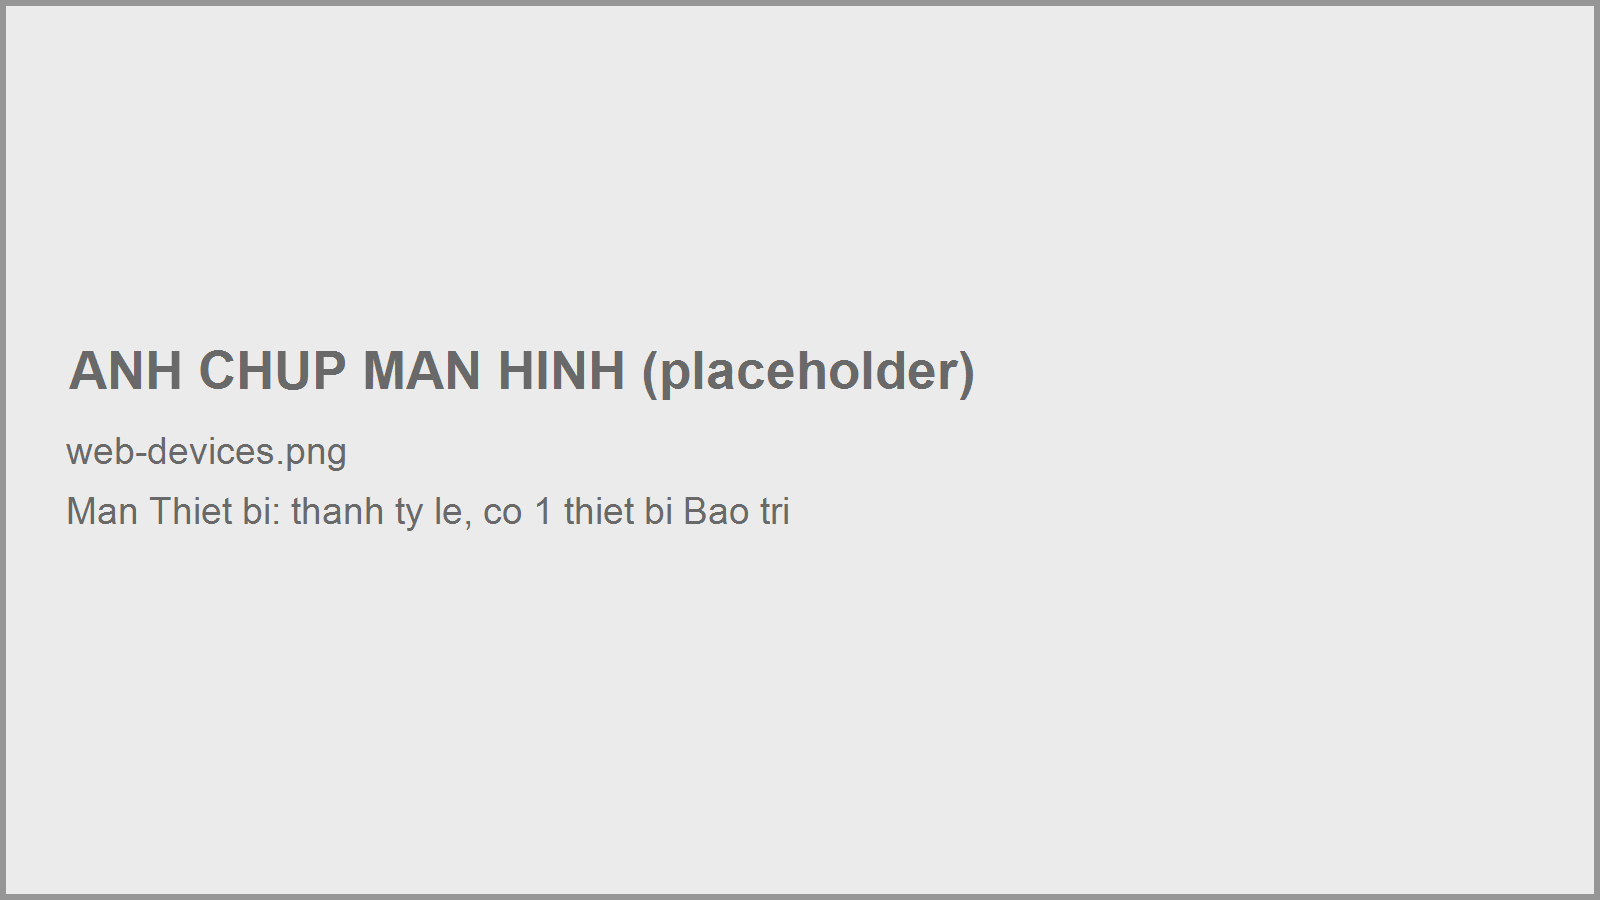
\includegraphics[width=0.95\textwidth]{figures/web-devices.png}
\caption{Màn Thiết bị: thanh tỷ lệ và trạng thái}
\label{fig:devices}
\end{figure}

\subsection{Mượn và gợi ý}
Chọn thiết bị vào giỏ; khung ``Thường được mượn kèm'' gợi ý theo cả giỏ (\code{suggestForBasket}) và tính lại mỗi khi thêm món.
\begin{figure}[H]
\centering
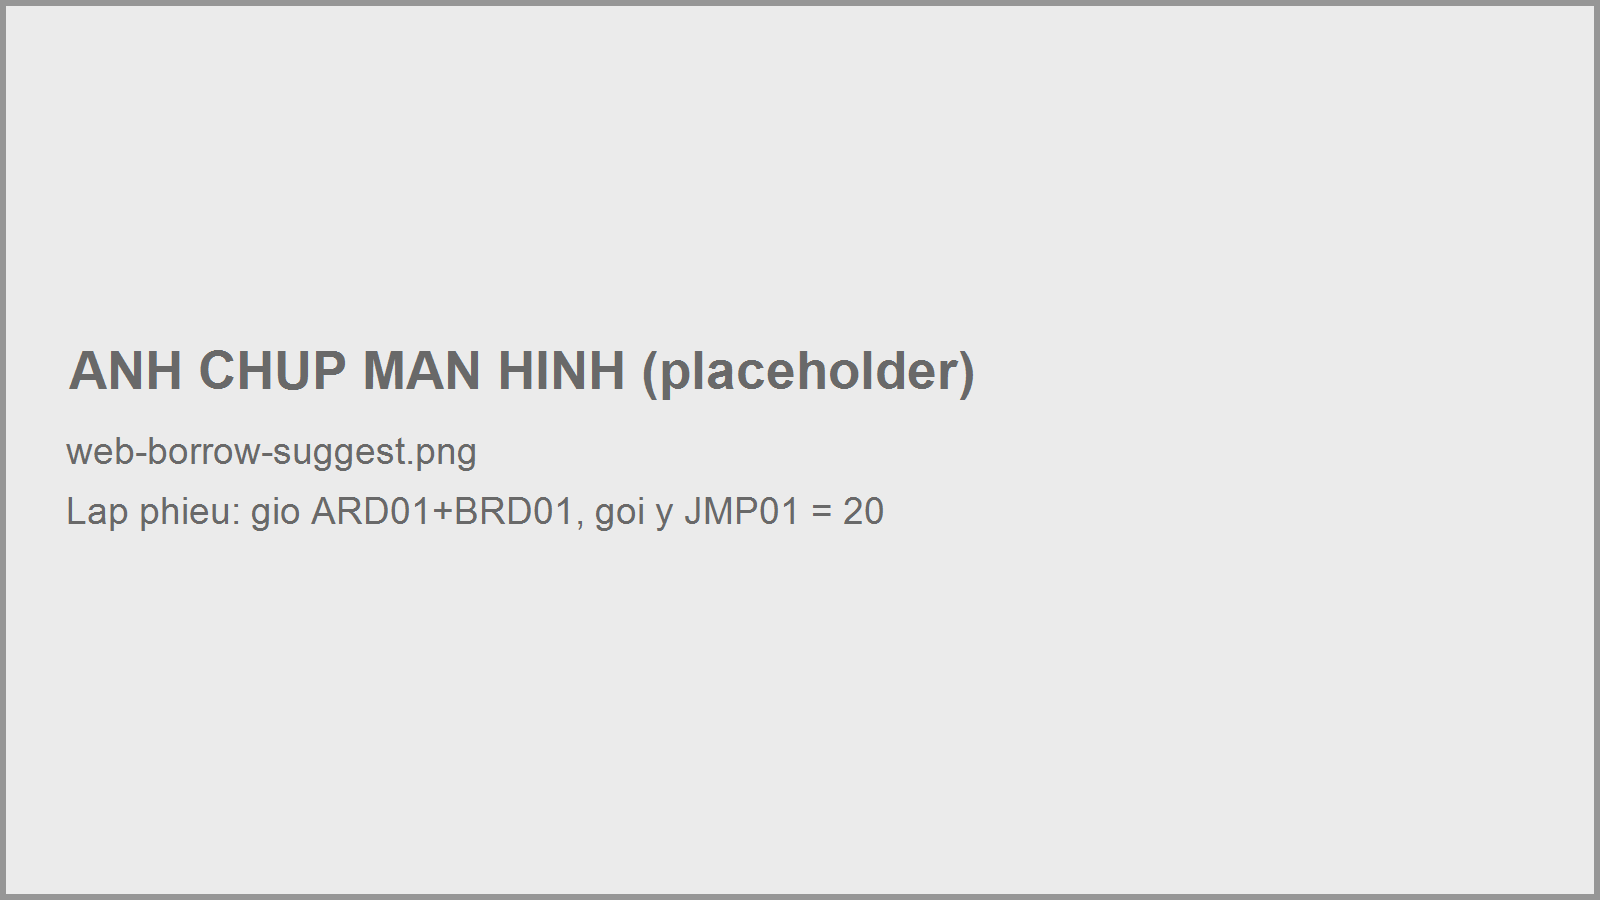
\includegraphics[width=0.95\textwidth]{figures/web-borrow-suggest.png}
\caption{Lập phiếu: giỏ ARD01 + BRD01, JMP01 đứng đầu với điểm cộng dồn 20}
\label{fig:borrow}
\end{figure}

\subsection{Trả thiết bị}
\begin{figure}[H]
\centering
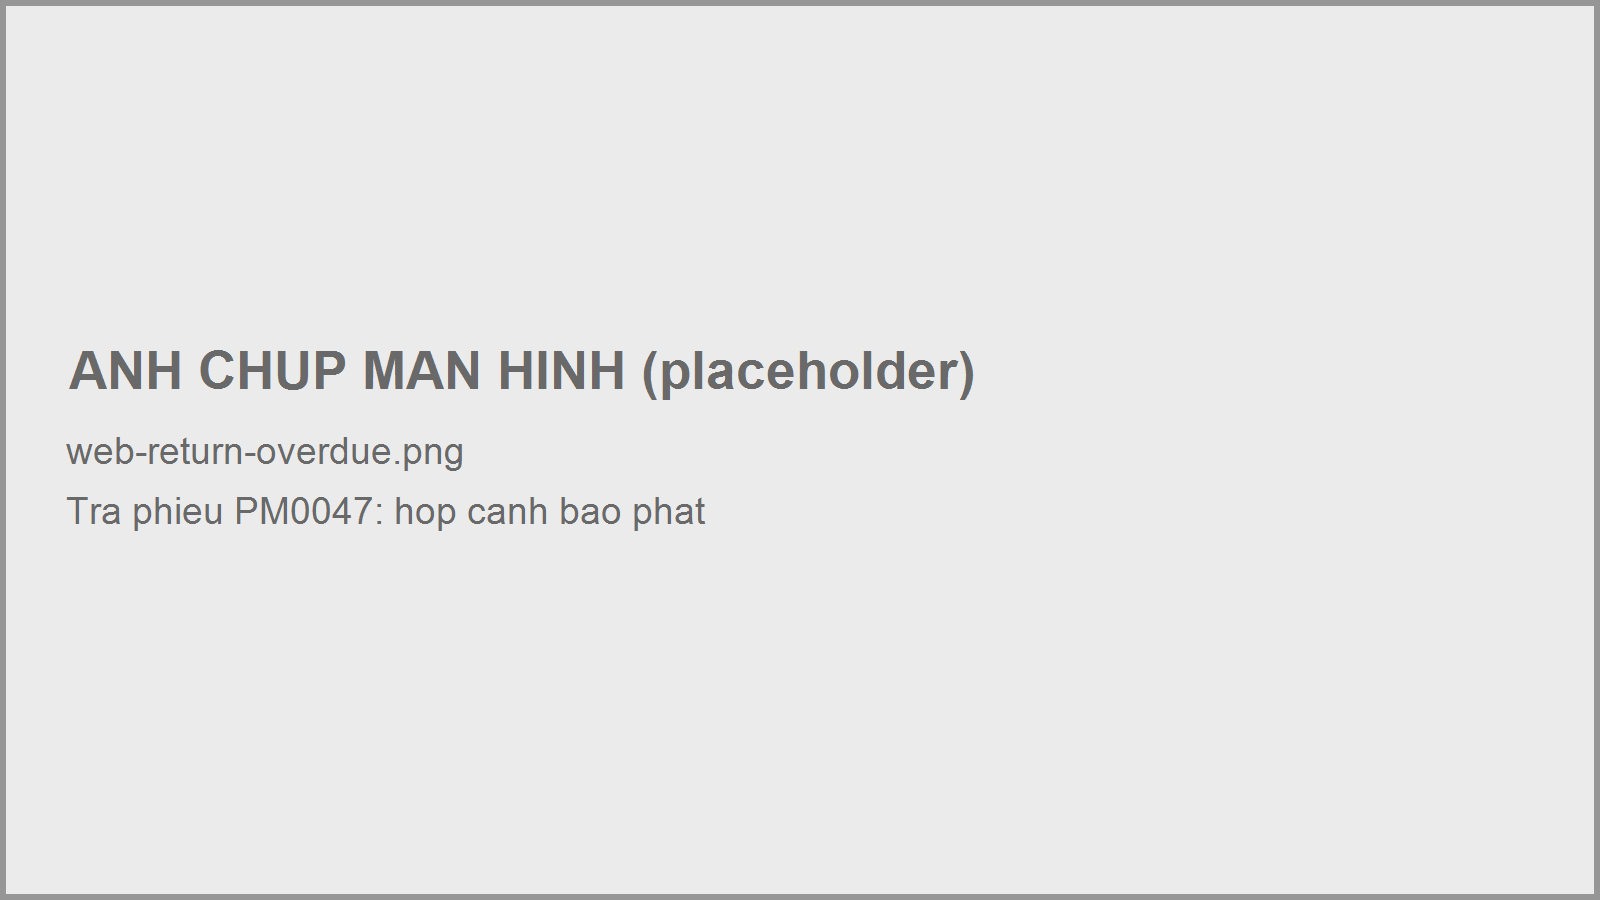
\includegraphics[width=0.95\textwidth]{figures/web-return-overdue.png}
\caption{Trả phiếu quá hạn: số ngày trễ và tiền phạt}
\label{fig:return}
\end{figure}

\subsection{Hàng đợi đặt trước}
Mỗi thiết bị một hàng: vị trí, trạng thái chờ/đang giữ, vòng đếm ngược 24 giờ, số lần lỡ hạn.
\begin{figure}[H]
\centering
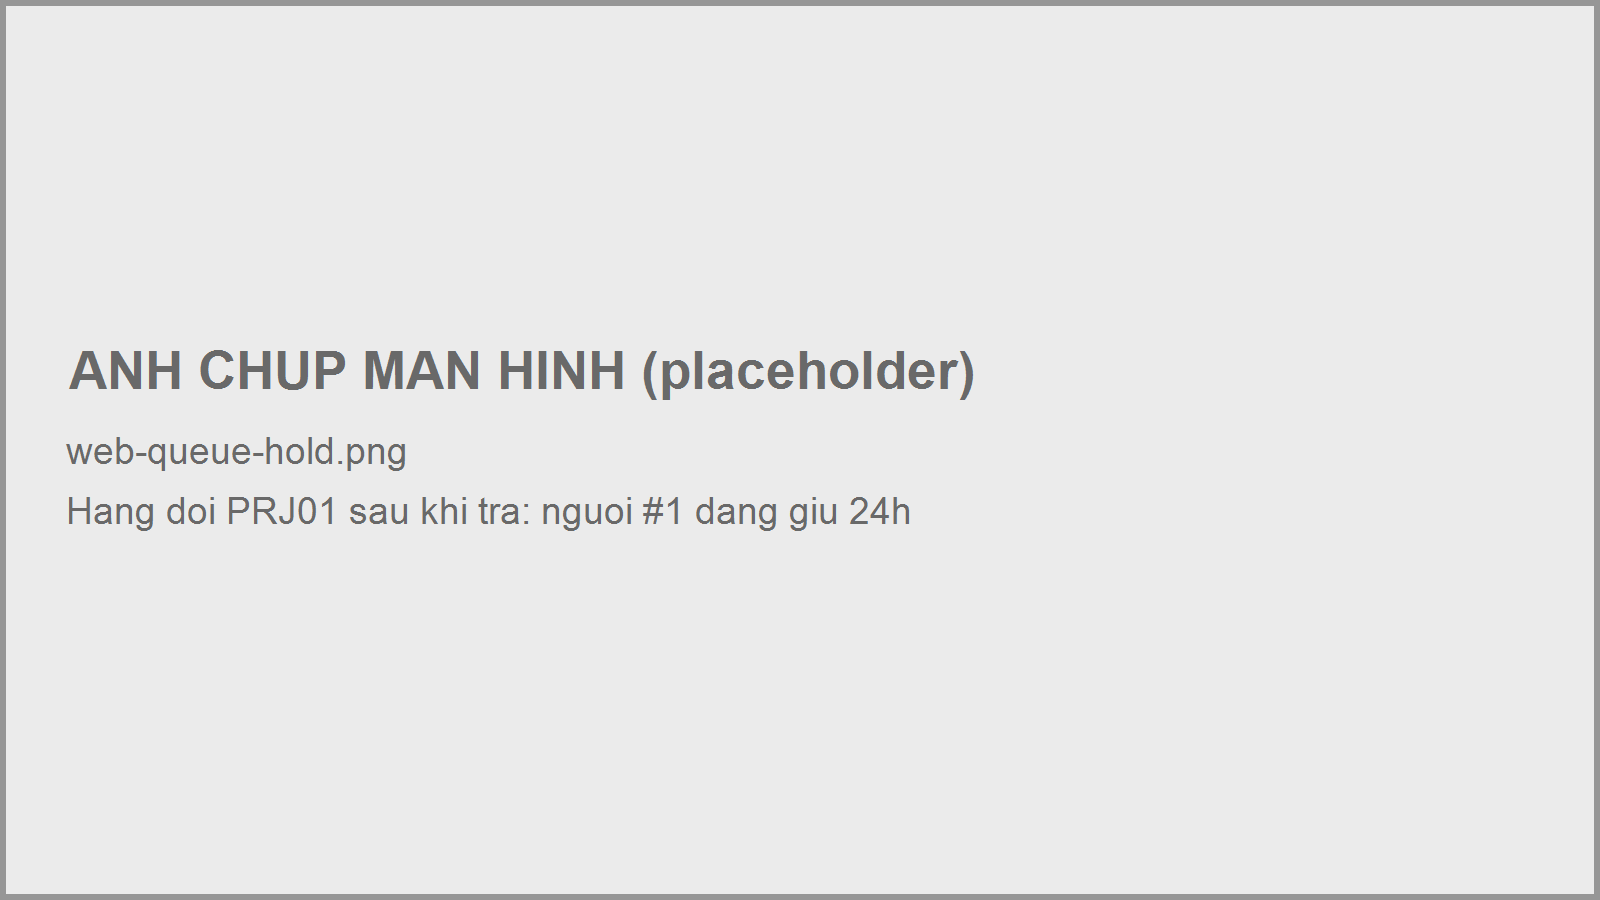
\includegraphics[width=0.95\textwidth]{figures/web-queue-hold.png}
\caption{Hàng đợi PRJ01 sau khi trả: người đứng đầu được giữ 24 giờ}
\label{fig:queue-hold}
\end{figure}
\begin{figure}[H]
\centering
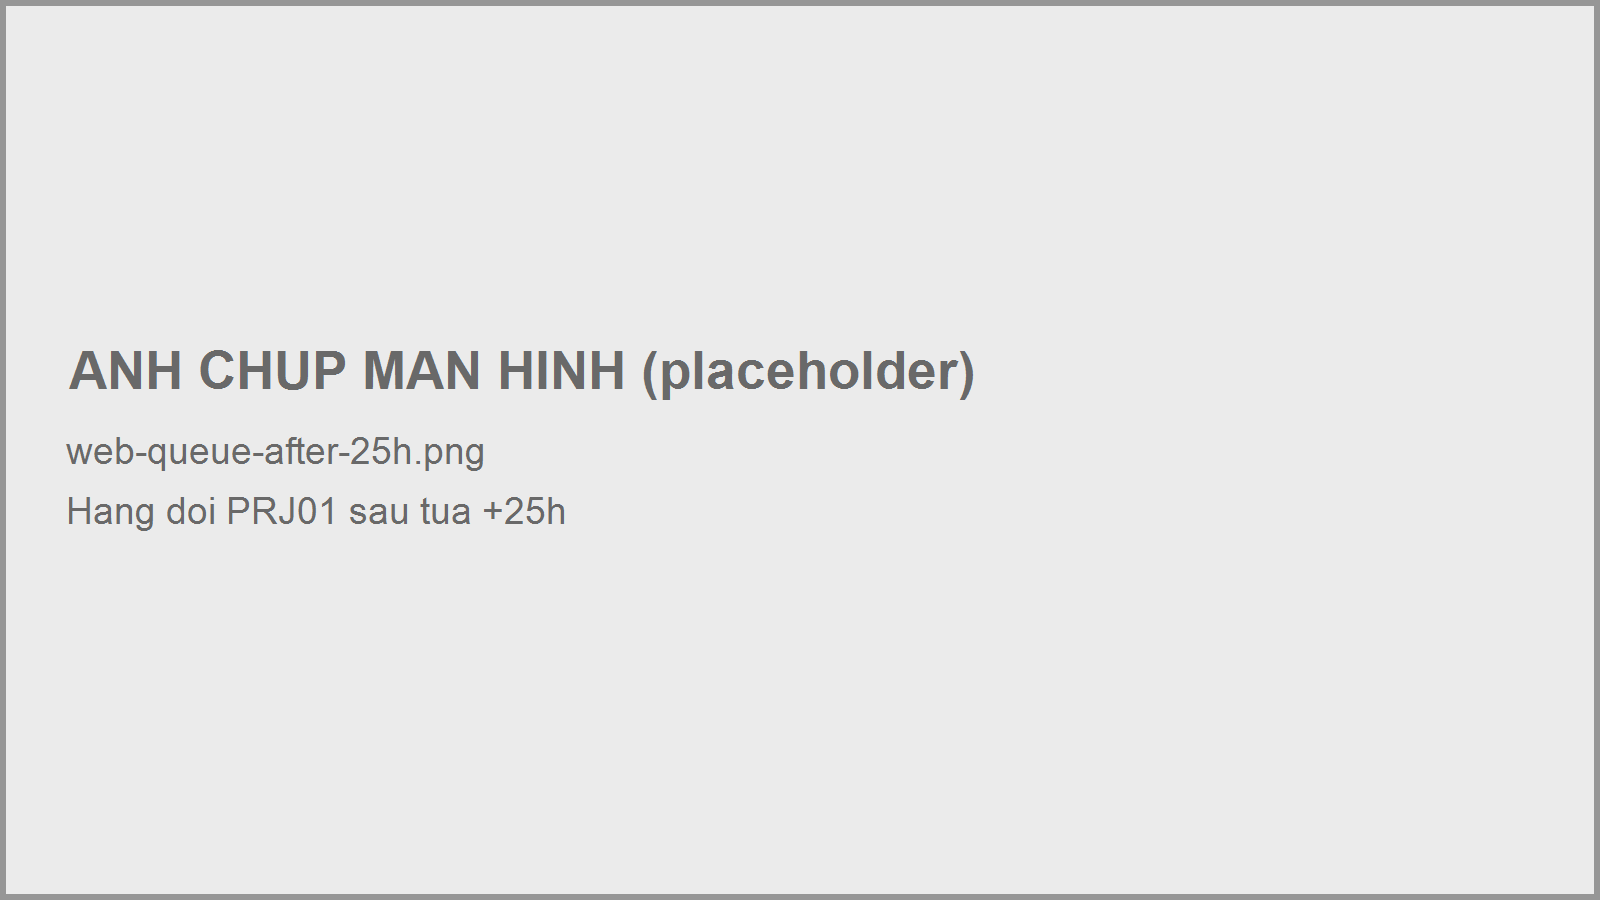
\includegraphics[width=0.95\textwidth]{figures/web-queue-after-25h.png}
\caption{Sau khi tua $+25$ giờ: người đầu lỡ hạn bị đẩy xuống cuối, người kế được giữ (hạn tính từ mốc cũ)}
\label{fig:queue-25h}
\end{figure}

\subsection{Quá hạn và lịch sử}
\begin{figure}[H]
\centering
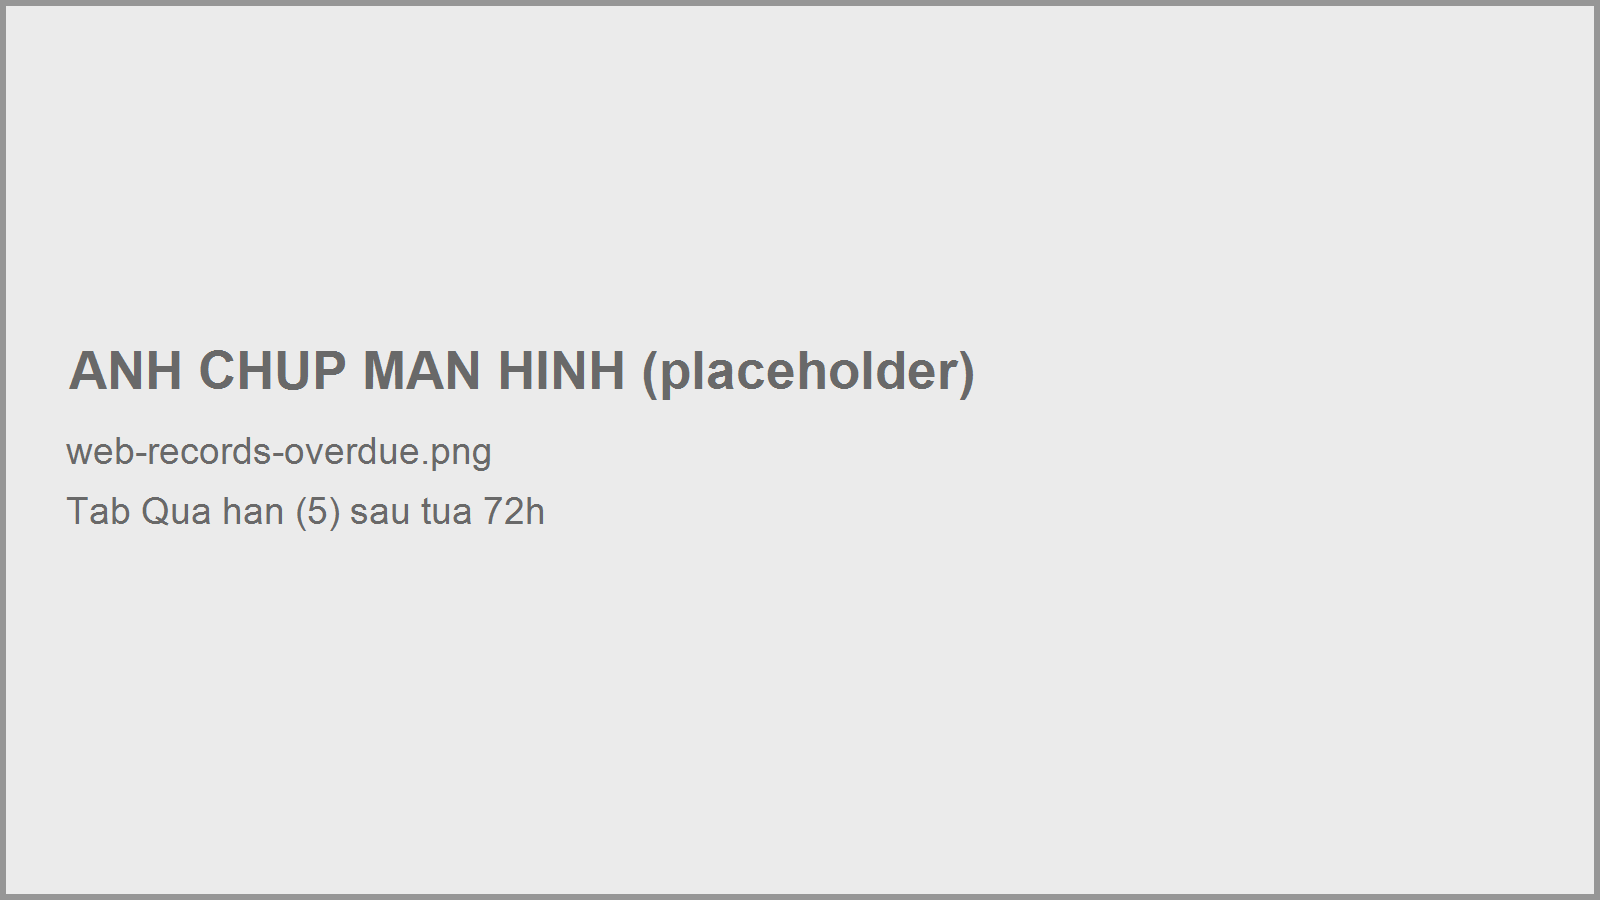
\includegraphics[width=0.95\textwidth]{figures/web-records-overdue.png}
\caption{Tab Quá hạn sau khi tua 72 giờ}
\label{fig:records}
\end{figure}

\subsection{Đồ thị mượn kèm}
Vẽ đồ thị với độ dày cạnh theo trọng số, lọc theo ngưỡng trọng số; chọn một đỉnh để xem top 3 mượn kèm.
\begin{figure}[H]
\centering
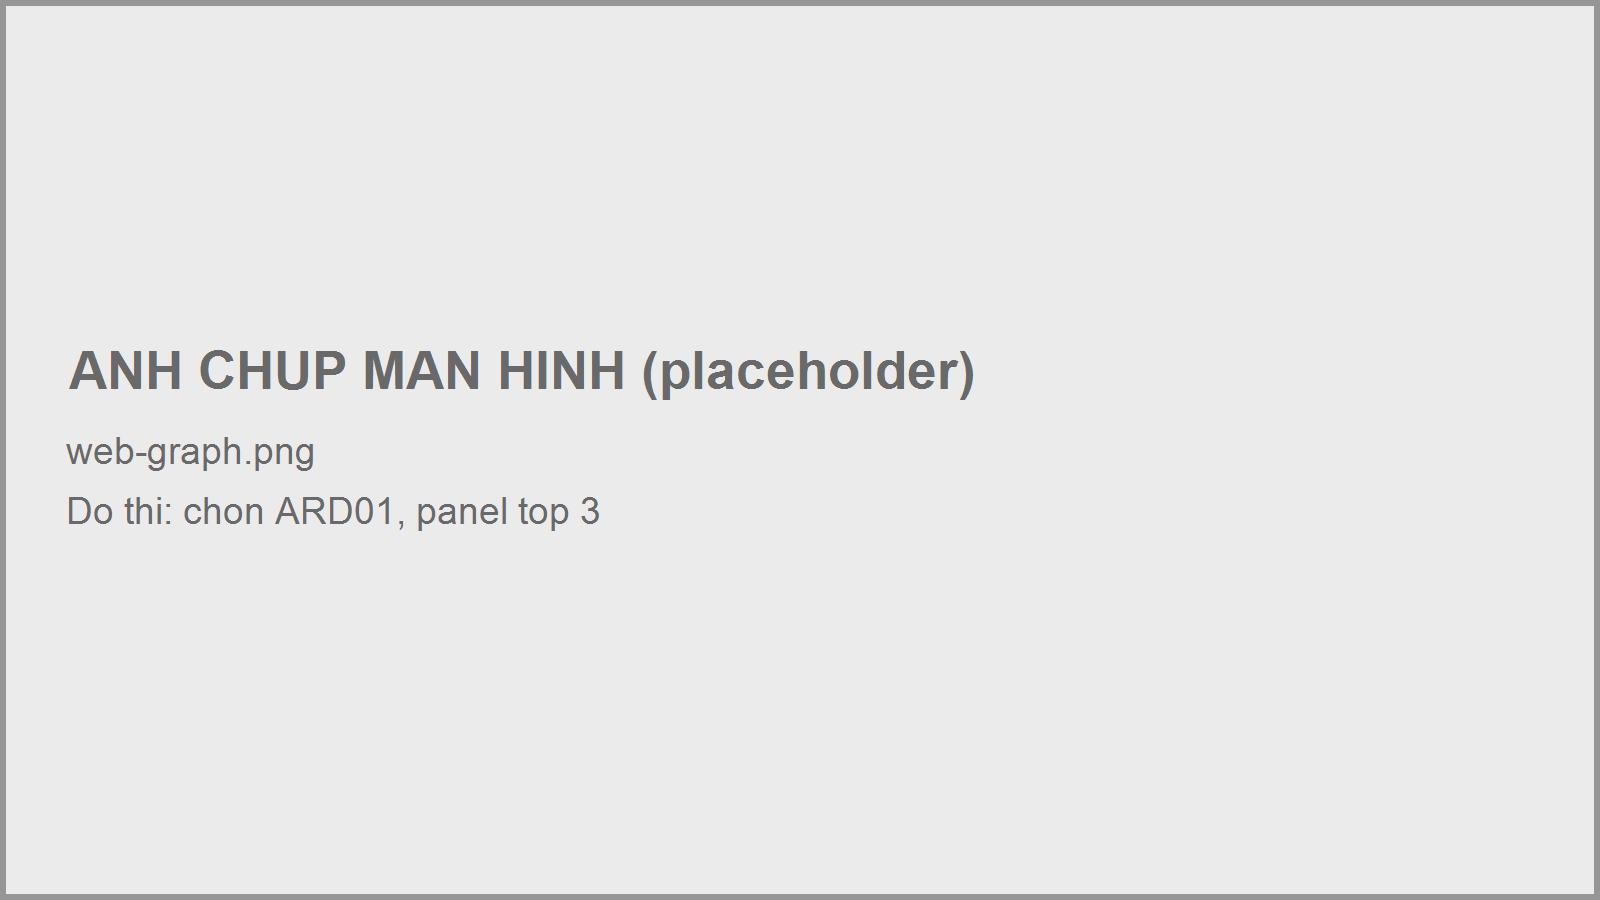
\includegraphics[width=0.95\textwidth]{figures/web-graph.png}
\caption{Màn đồ thị: chọn ARD01, panel top 3 thiết bị mượn kèm}
\label{fig:graph-ui}
\end{figure}
